\providecommand{\main}{..}
% \documentclass[\main/thesis.tex]{subfiles}

\begin{document}
\chapter{The $n$-Step Q($\sigma$) Algorithm}
\label{ch3:qsigma}

In this chapter, we introduce the main algorithm to be studied in this thesis: $n$-step $Q(\sigma)$.
The $n$-step $Q(\sigma)$ algorithm will be the basis for the theoretical analyses in chapter \ref{ch4:convergence} and the empirical evaluations in chapter \ref{ch5:empirical_evaluation}.

We will start by introducing the $1$-step version of $Q(\sigma)$ and its extension to the off-policy setting.
We then continue to extend $1$-step $Q(\sigma)$ to the $n$-step case and show how it can represent the $n$-step algorithms Sarsa and tree backup, effectively unifying them under the same family of algorithms.
After introducing $n$-step $Q(\sigma)$, we will show its extension to the continuous case with linear function approximation in combination with the tile coding feature representation.
We will finish this chapter by extending the $n$-step $Q(\sigma)$ algorithm to the continuous case with non-linear function approximation.
We will achieve this last extension by modifying the DQN architecture \parencite{mnih2015humanlevel} so that it is able to use $n$-step $Q(\sigma)$ instead of $Q$-learning.
We have named this architecture the deep $Q(\sigma)$ network.

%%%%%%%%%% One-Step Q(Sigma) %%%%%%%%%%
\section{One-Step $Q(\sigma)$}

In essence, the one-step $Q(\sigma)$ algorithm is a convex combination of Sarsa and Expected Sarsa.
The parameter $\sigma$ lets us decide whether to use Sarsa and sample the next action-value estimate, or use Expected Sarsa and take an expectation over all the possible next action-value estimates.
If we choose $\sigma$ equal to one, we select Sarsa, whereas with $\sigma$ equal to zero, we select Expected Sarsa. 
Nevertheless, it is possible to select values of $\sigma$ anywhere in the interval $[0,1]$.
In this case, we give Sarsa a weight of $\sigma$ and Expected Sarsa a weight of $(1-\sigma)$.
The resulting estimate of the return is defined as
%
\begin{align}
\label{eq:1step_qsigma_return}
\hat{G}_t &\overset{.}{=} \sigma \big[ R_{t+1} + \gamma Q_t(S_{t+1}, A_{t+1}) \big] 
	+ (1-\sigma) \big[ R_{t+1} + \gamma \sum_{a \in \mathcal{A}} \pi(a|S_{t+1}) Q_t(S_{t+1}, a) 
    \big] \nonumber \\
%
&= R_{t+1} + \gamma \big[ \sigma Q_t(S_{t+1}, A_{t+1}) + (1-\sigma) \sum_{a \in \mathcal{A}} Q_t(S_{t+1}, a) \big].
\end{align}
%
We can then use the update function from the previous chapter
%
\begin{align}
\label{eq:av_update}
Q_{t+1}(S_t,A_t) = (1-\alpha) Q_t(S_t, A_t) + \alpha \hat{G}_{t},
\end{align}
%
in order to iteratively compute the estimates of the action-value function.

Just like the Sarsa and Expected Sarsa algorithms, we can represent the $Q(\sigma)$ algorithm using a backup diagram.
In this case, we can choose from two different graphical representations. 
Figure (\ref{fig:qsigma_backup}a), represents the one-step $Q(\sigma)$ algorithm as a convex combination of the backup diagrams corresponding to Sarsa and Expected Sarsa, where Sarsa is weighted by $\sigma$ and Expected Sarsa is weighted by $(1-\sigma)$.
On the other hand, figure (\ref{fig:qsigma_backup}b) represents our algorithm as a single backup diagram with two separate paths: a sampling path weighted by $\sigma$ and an expectation path weighted by $(1-\sigma)$. 
The dashed lines in the diagram connecting two solid dots indicate that those actions or state-action pairs are the same in both sides of the diagram.
We will demonstrated in the next section that the $n$-step $Q(\sigma)$ algorithm can always be represented as a convex combination of $2^n$ different diagrams.
Hence, I advocate for the backup diagram in figure (\ref{fig:qsigma_backup}b) since it is more compact and conveys the same amount of information.

\begin{figure}
    \centering
    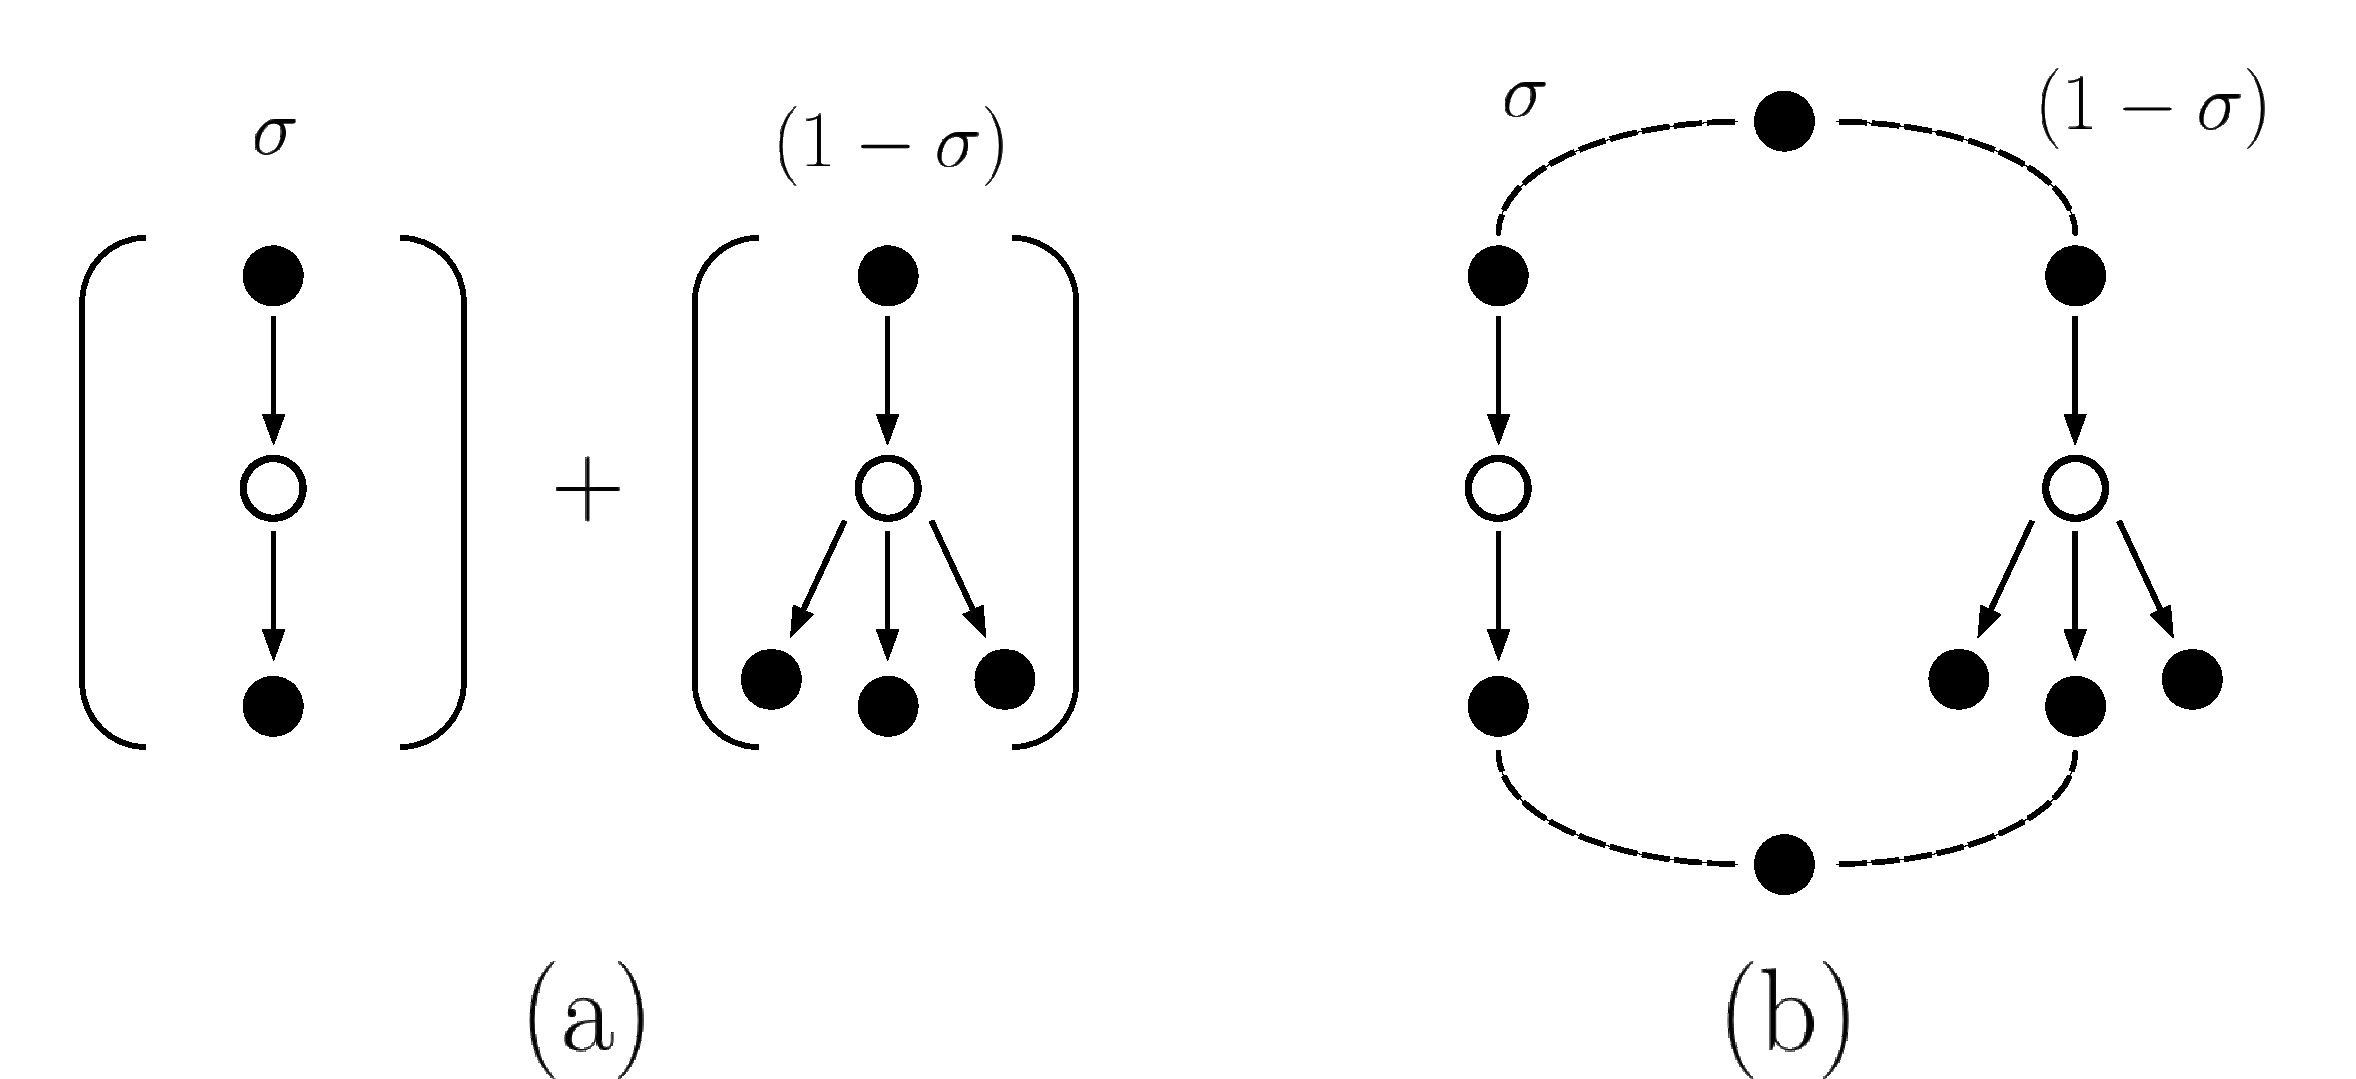
\includegraphics[keepaspectratio=true, width=1\textwidth]{\main/img/qsigma_backup}
    \caption[One-Step Q(Sigma) Backup Diagram] {
    Two Graphical Representations of the one-step $Q(\sigma)$ algorithm. 
    Diagram (a) represents $Q(\sigma)$ as a convex combination of Sarsa and Expected Sarsa, each
    with weights $\sigma$ and $(1-\sigma)$, respectively.
    Diagram (b) represents $Q(\sigma)$ as a single diagram with a sampling path weighted by $\sigma$
    and an expectation path weighted by $(1-\sigma)$.
    The dashed lines connecting two solid dots indicate that both actions or state-action pair are
    the same in both sides of the backup.
    }
    \label{fig:qsigma_backup}
\end{figure}

As we can observe in figure (\ref{fig:qsigma_backup}), the parameters $\sigma$ allows us to represent a wide variety of algorithms while subsuming the existing one-step algorithms as special cases.
Moreover, the parameter $\sigma$ need not to remain constant over time and can be made a function of the current state at time $t$.
We can rewrite the return in equation (\ref{eq:1step_qsigma_return}) to extend the parameter $\sigma$ to these two special cases.
%
\begin{align}
& \hat{G}_t \overset{.}{=} R_{t+1} + \gamma \big[ \sigma_{t+1}(S_{t+1}) Q_t(S_{t+1}, A_{t+1}) 
	\nonumber \\
& \hspace{80pt} 
	+ (1-\sigma_{t+1}(S_{t+1})) \sum_{a \in \mathcal{A}} \pi(a|S_{t+1}) Q_t(S_{t+1}, a) \big].
\end{align}
%
Additionally, $\sigma$ can also be made a function of the current action $A_{t+1}$.
However, we restrain from this generalization since the convergence results presented in the next section do not apply to this special case.
Henceforth, we will denote the $\sigma$ parameter as $\sigma_t$ to indicate that it is a function of the time $t$, but with the understanding that $\sigma$ can also be a extended to be a function of the state.

Finally, one-step $Q(\sigma)$ can be extended to the off-policy case by using the importance sampling ratio, $\rho_{t+1} = \frac{\pi(A_{t+1}|S_{t+1})}{\mu(A_{t+1}|S_{t+1})}$, where $\pi$  is the target policy and  $\mu$ is the behaviour policy.
The resulting estimate of the return is
%
\begin{equation}
\label{eq:offpolicy_1step_qsigma_return}
\hat{G}_t \overset{.}{=} R_{t+1} + \gamma \big[\sigma_t \rho_{t+1} Q(S_{t+1}, A_{t+1}) 
	+ (1-\sigma_t) \sum_{a \in \mathcal{A}} \pi(a|S_{t+1}) Q_{t}(S_{t+1}, a) \big].
\end{equation}
%
We can then compute estimates of the action-value by plugging in the estimate of the return in equation (\ref{eq:offpolicy_1step_qsigma_return}) into the update function in equation (\ref{eq:av_update}).
Note that the Expected Sarsa side of the return does not need importance sampling since it is already computing the expected value of the action-value function under the target policy.


%%%%%%%%%% n-Step Q(Sigma) %%%%%%%%%%
\section{$n$-Step $Q(\sigma)$}

Just like Sarsa and Expected Sarsa, $Q(\sigma)$ can be extended to the $n$-step case where, instead of looking one step into the future, we look several steps into the future in order to compute an update.
In the $n$-step case, $Q(\sigma)$ effectively unifies the $n$-step Sarsa and $n$-step Tree Backup algorithms.
In this case, it will be more intuitive to introduce the algorithm graphically using backup diagrams.

\begin{wrapfigure}{l}{0.6\textwidth}
  \begin{center}
    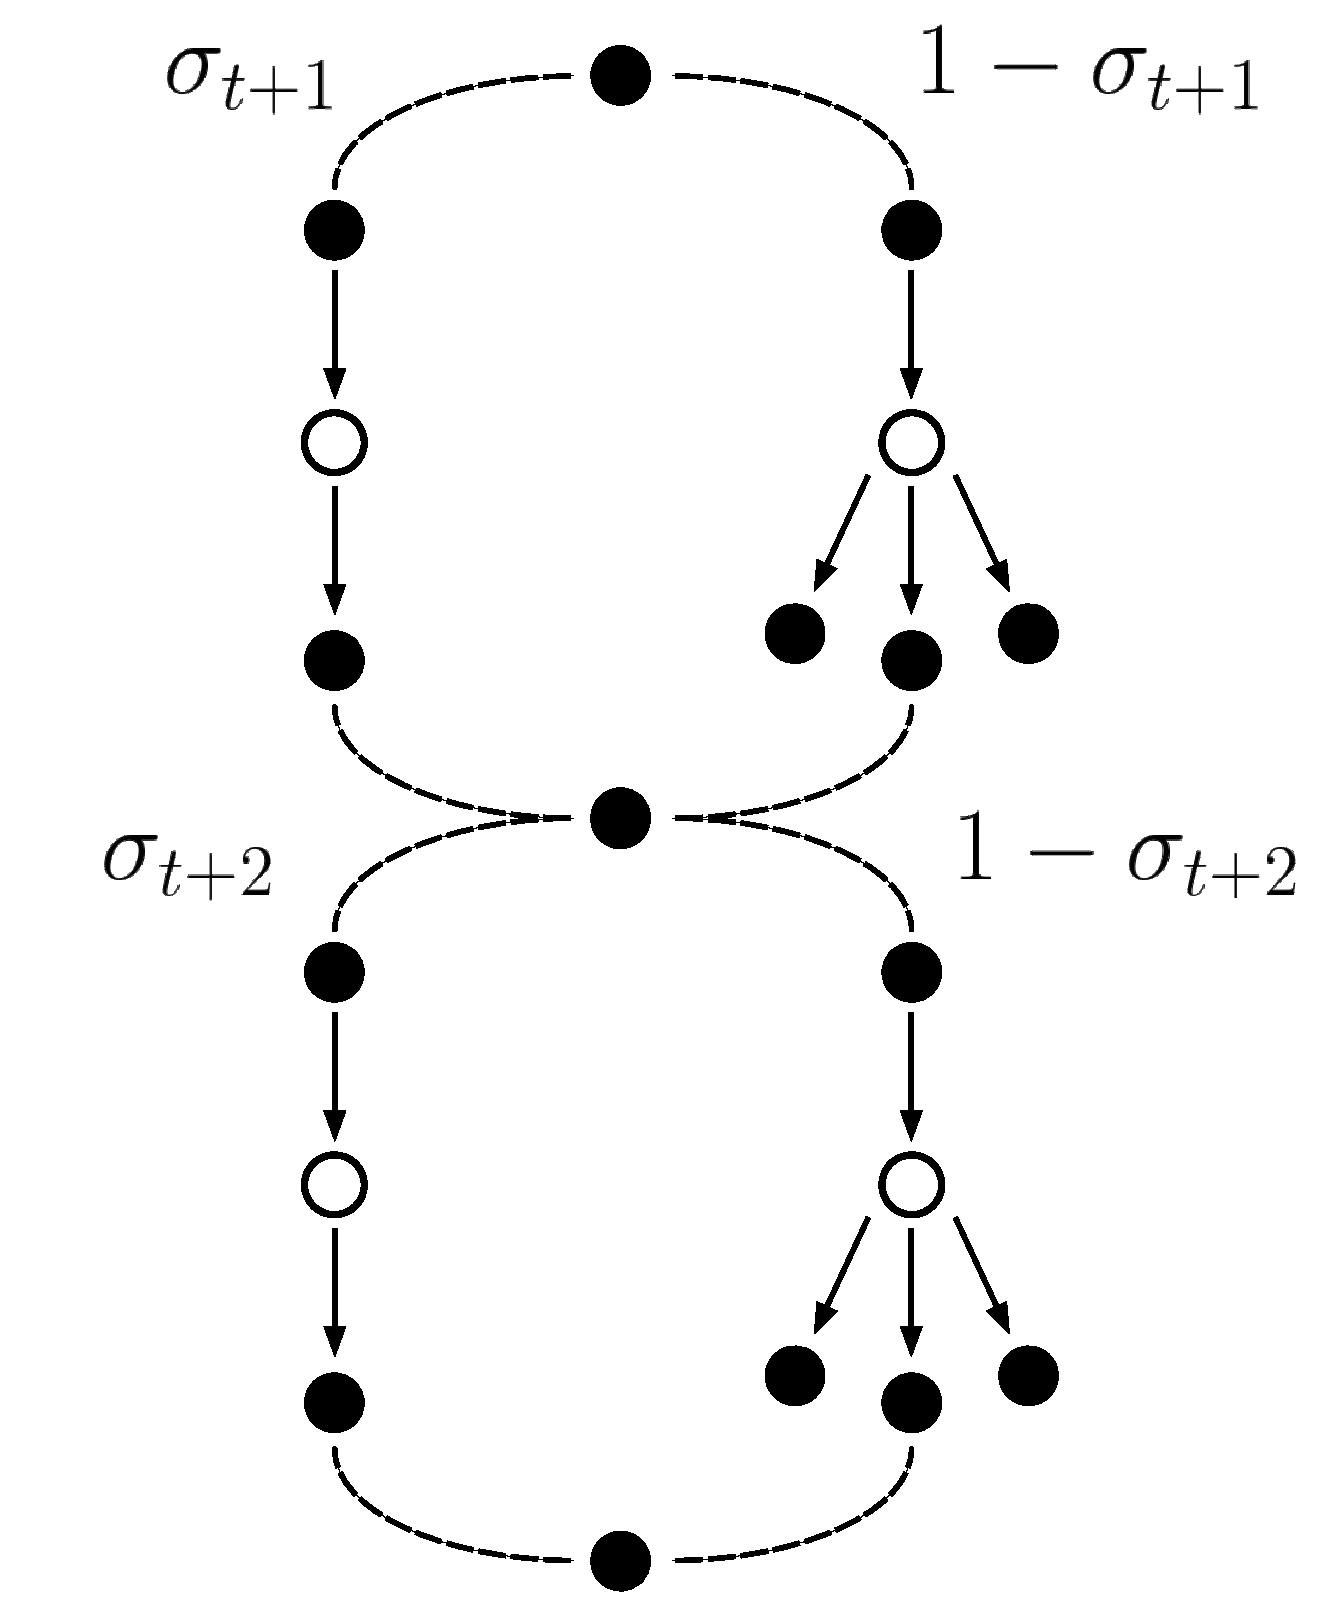
\includegraphics[keepaspectratio=true, width=0.55\textwidth]{\main/img/2step_qsigma_backup}
  \end{center}
  \caption{Two-Step $Q(\sigma)$ Backup Diagram}
  \label{fig:nstep_qsigma_backup}
\end{wrapfigure}

Figure (\ref{fig:nstep_qsigma_backup}) shows the backup diagram of the two-step $Q(\sigma)$ algorithm.
At each step of the diagram we can can choose between sampling the next state-action pair or taking an expectation over all the possible state-action pairs.
At every timestep $t + k$, for $k \geq 1$, the sampling path is weighted by $\sigma_{t + k}$, whereas the expectation path is weighted by $(1-\sigma_{t + k})$.

The two-step $Q(\sigma)$ algorithm can also be interpreted as a convex combination of several backup diagrams as shown in figure (\ref{fig:twostep_qsigma_convex_comb}).
The weights corresponding to each of the backup diagrams is listed above their corresponding diagram.
Thus, for a backup length of $n$, the $n$-step $Q(\sigma)$ algorithm is a convex combination of $2^n$ different backup diagrams.
Note that, even for a small value of $n$, it quickly becomes inconvenient to represent the $n$-step $Q(\sigma)$ algorithm as a convex combination of several different backups.
Hence, I advocate for the graphical representation presented in figure (\ref{fig:nstep_qsigma_backup}) since it is more compact while conveying the same amount of information.
It is clear from figure (\ref{fig:twostep_qsigma_convex_comb}) that if we choose a fixed value of $\sigma$ of one, we recover two-step Sarsa, whereas with a fixed value of $\sigma$ of zero we recover two-step Tree Backup.

\begin{figure}[t]
    \centering
    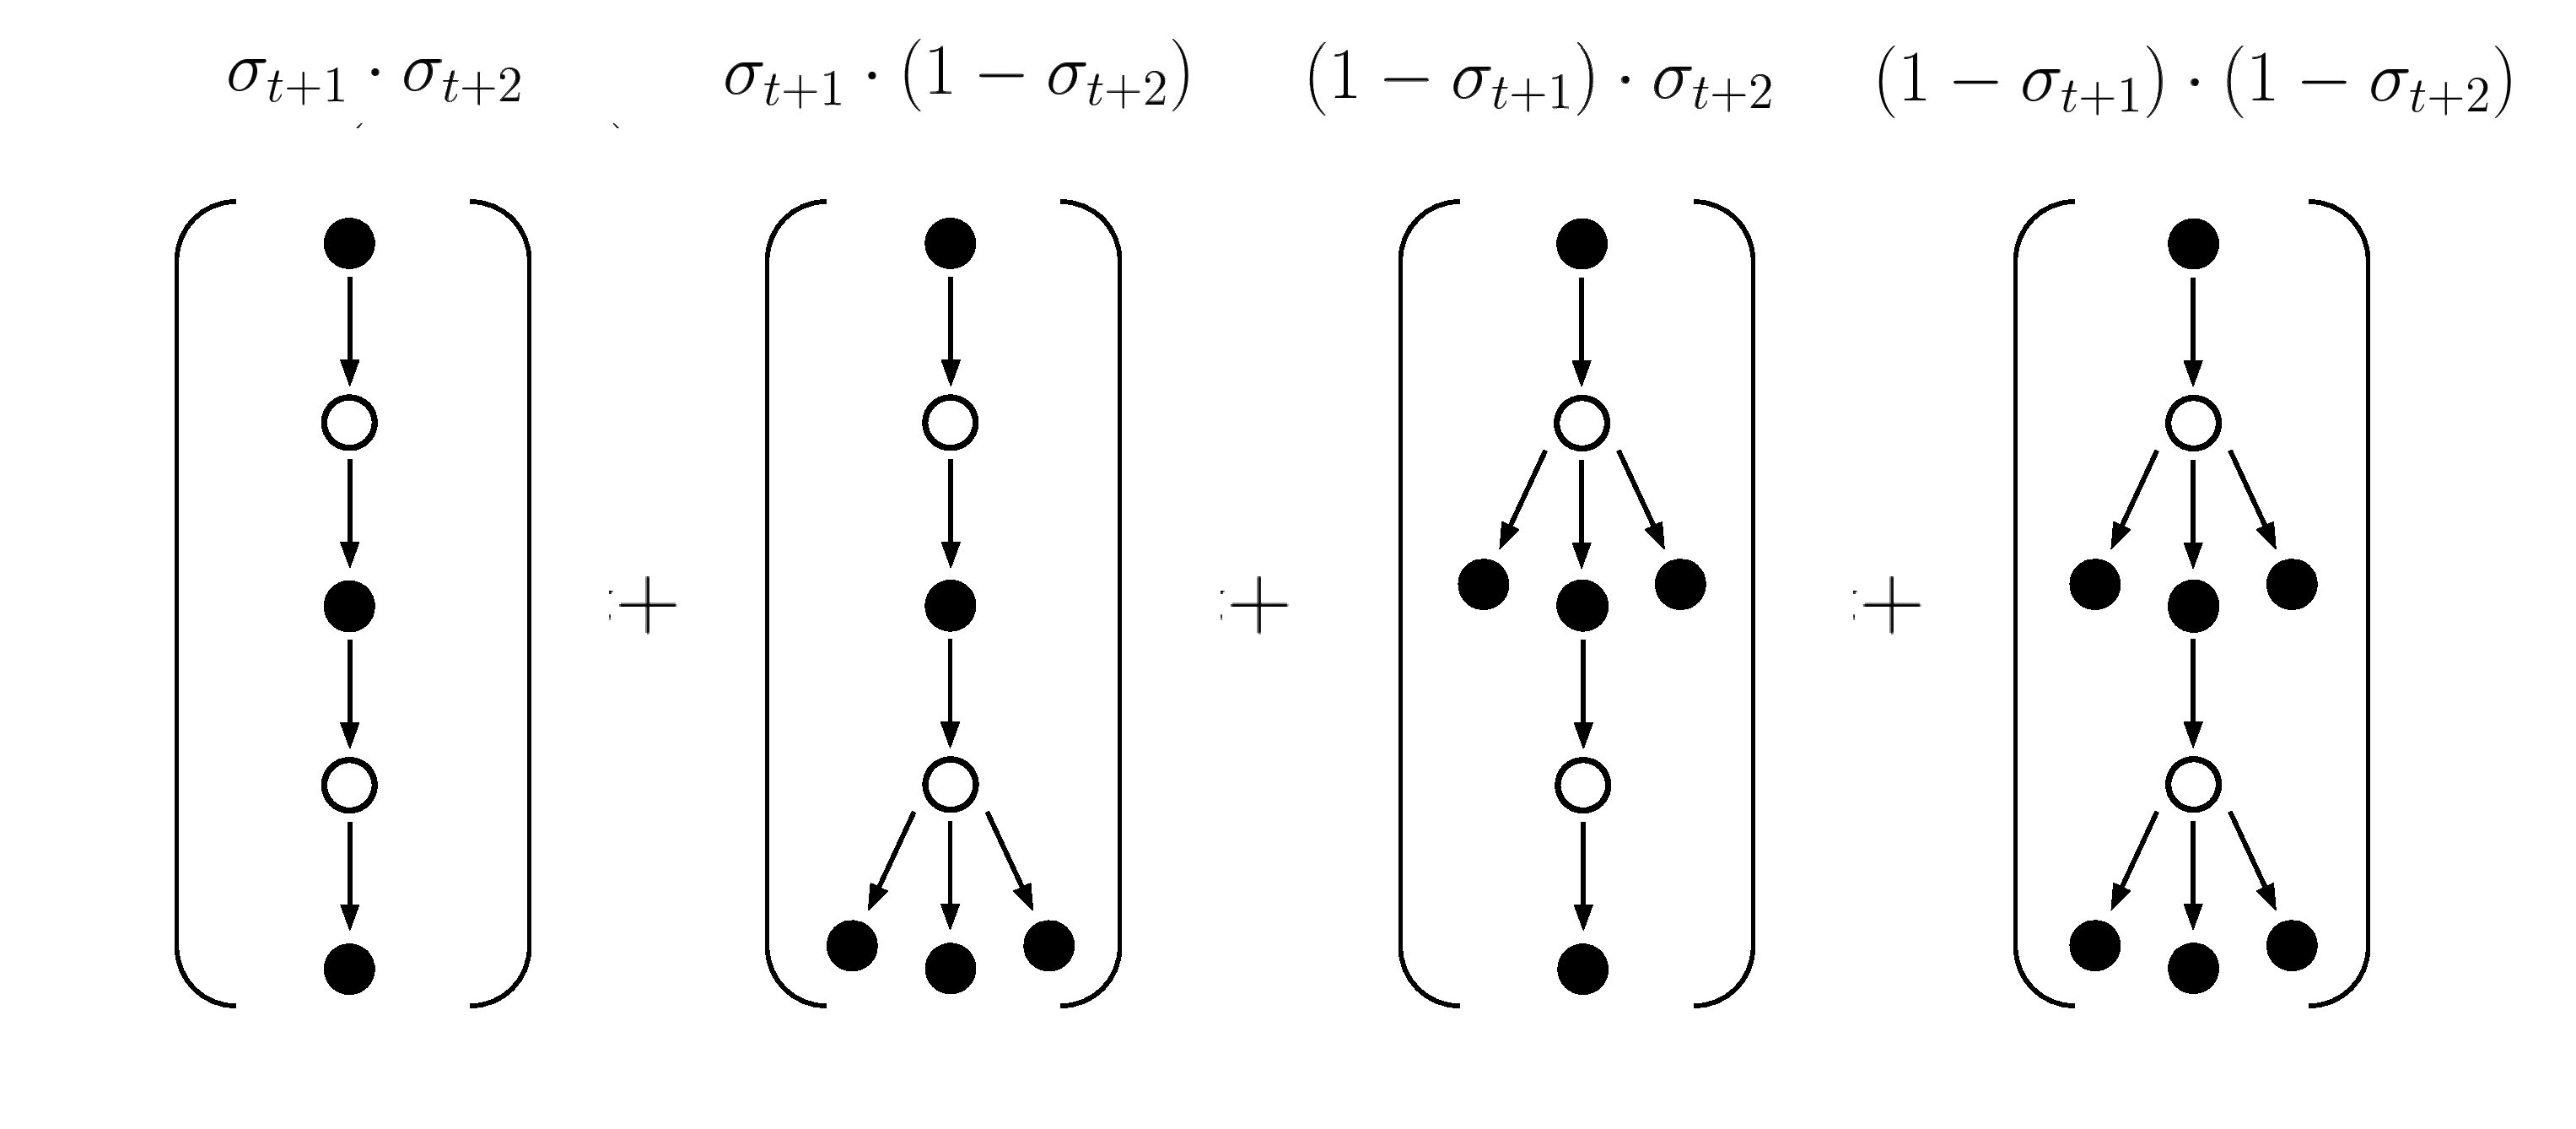
\includegraphics[keepaspectratio=true, width=1\textwidth]{\main/img/2step_qsigma_convex_combination}
    \caption[Two-Step Q(Sigma) as a Convex Combination] {
    Two-step $Q(\sigma)$ backup represented as a convex combination of four
    different backups.
    The weight assigned to each backup is written above the corresponding backup diagram.
    } 
    \label{fig:twostep_qsigma_convex_comb}
\end{figure}

In order to implement the $n$-step $Q(\sigma)$ algorithm with time-dependent $\sigma$, we use the estimate of the return
%
\begin{align}
\label{eq:nstep_qsigma_return}
\hat{G}_{t:t+n} &\overset{.}{=} \sum_{k=0}^{n-1} \gamma^{k}  
	\big(\prod_{s=1}^{k} C_{t+s}\big) \big[R_{t+1+k} \nonumber  \\
& \hspace{30pt} +\gamma (1-\sigma_{t+1+k}) \sum_{a\in\mathcal{A}}\mathbb{I}\{a \neq A_{t+1+k}\} 
	\pi(a|S_{t+1+k}) Q_{t+k}(S_{t+1+k},a) \big] \nonumber \\
& \hspace{30pt} +\gamma^n \big(\prod_{s=1}^{n} C_{t+s}\big) Q_{t+n-1}(S_{t+n}, A_{t+n}),
\end{align}
%
where $C_t = \sigma_{t} + (1-\sigma_t)\pi(A_t|S_t)$ and $\mathbb{I}\{ \cdot \}$ is an indicator variable which is equal to one when the statement in brackets is true and equal to zero otherwise. 
Additionally, the product term $\prod$ is defined as one when there are no elements inside of it.

In this case, the recursive definition of the estimate of the return is less convoluted and it is defined as
%
\begin{align}
\label{eq:recursive_nstep_return}
%% line 1
\hat{G}_{t:t+n} &\overset{.}{=} R_{t+1} + \big[ \sigma_{t+1} + (1-\sigma_{t+1})\pi(A_{t+1}|S_{t+1}) \big]
	\hat{G}_{t+1:t+n} \nonumber \\
%% line 2
&\hspace{15pt}
	+ (1-\sigma_{t+1}) \sum_{a \in \mathcal{A}} \mathbb{I}\{ a \neq A_{t+1} \} \pi(a|S_{t+1}) 
	Q_{t+n-1}(S_{t+1}, a),
	\nonumber \\
%% line 3: base case
\hat{G}_{t+n:t+n} &\overset{.}{=} Q_{t+n-1}(S_{t+n}, A_{t+n}).
\end{align}
%
The recursive definition above illustrates better the idea of choosing between sampling and taking an expectation at every step.
At timestep $t+k$, for $n \geq k \geq 1$, we can choose to take an expectation over $\hat{G}_{t+k:t+n}$ and all the other action-value estimates if we let $\sigma_{t+k}$ be zero.
Otherwise, we can choose to keep unrolling $\hat{G}_{t+k:t+n}$ by letting $\sigma_{t+k}$ be equal to one. 

Note that the samples needed to compute the estimate of the return are not available until time $t+n$.
Consequently, the update for the action-value estimate corresponding to $(S_t, A_t)$ can only be computed at time $t+n$.
This results in the $n$-step update function from the previous chapter
%
\begin{equation}
\label{eq:general_nstep_update}
Q_{t+n}(S_t, A_t) = (1-\alpha)Q_{t+n-1}(S_t,A_t) + \alpha \hat{G}_{t:t+n}.
\end{equation}
As a consequence, the agent does not benefit from any learning during the first $n$ timesteps of an episode.

Just like in the one-step case, we can extend the $n$-step $Q(\sigma)$ algorithm to the off-policy setting via importance sampling.
To do so we can let $C_t = \sigma_t \rho_t + (1-\sigma_t)\pi(A_t|S_t)$ in equation (\ref{eq:nstep_qsigma_return}), or we can modify equation (\ref{eq:recursive_nstep_return}) to include the importance sampling term:
%
\begin{align}
\label{eq:offpolicy_recursive_nstep_return}
\hat{G}_{t:t+n} &\overset{.}{=} R_{t+1} + \big[ \sigma_{t+1} \rho_{t+1} + (1-\sigma_{t+1})\pi(A_{t+1}|S_{t+1}) \big]
	\hat{G}_{t+1:t+n} \nonumber \\
%
& \hspace{15pt}
	+ (1-\sigma_{t+1}) \sum_{a \in \mathcal{A}} \mathbb{I}\{ a \neq A_{t+1} \} \pi(a|S_{t+1}) 
    Q_{t}(S_{t+1}, a),
\end{align}
%
where $\rho_{t+1} = \frac{\pi(A_{t+1}|S_{t+1})}{\mu(A_{t+1}|S_{t+1})}$.
The update is computed by substituting the estimate of the return in the update function in equation (\ref{eq:general_nstep_update}) with the estimate of the return in equation (\ref{eq:offpolicy_recursive_nstep_return}).

The algorithm box below shows the pseudocode for the off-policy $n$-step $Q(\sigma)$.
Note that the update is implicitly assuming that $Q_{t+1}(s,a) \overset{.}{=} Q_t(s,a)$ for all state-action not equal to $(S_\tau, A_\tau)$.

\begin{algorithm}[H]
	\caption{Off-policy $n$-step $Q(\sigma)$}
	\label{alg:tabular_nstep_qsigma}
	\begin{algorithmic}[1]
    	\STATE Input: a behaviour policy $\mu$ such that $\mu(a|s) > 0$ for all 
        		$(s,a) \in \mathcal{S} \times \mathcal{A}$
		\STATE Initialize $Q_0(s,a)$ arbitrarily for all $(s,a) \in \mathcal{S} \times \mathcal{A}$
        \STATE Initialize the target policy $\pi$ as a function of $Q$ or as fixed policy
        \STATE Algorithm Parameters: learning rate $\alpha \in (0,1]$, backup length $n$
        \FOR{Every Episode}
        	\STATE Initialize $S_0$, select $A_0 \sim \mu(\cdot | S_0)$
            \STATE Store $S_0$ and $A_0$
            \STATE Initialize $T \leftarrow \infty$; $t \leftarrow 0$
            \WHILE{$t < T + n$}
            	\IF{$t < T$}
            		\STATE Take action $A_t$; observe and store $R_{t+1}$ and $S_{t+1}$
                	\IF{$S_{t+1}$ is terminal}
                		\STATE $T \leftarrow t+1$
					\ELSE
                      	\STATE Choose and store action $A_{t+1} \sim \mu(\cdot| S_{t+1})$ and 
                        	$\sigma_{t+1}$
                  	\ENDIF
                \ENDIF
                \STATE $\tau \leftarrow t + 1 - n$ ($\tau$ is the time whose estimate is being
                		updated)
                \IF{$\tau \geq 0$}
                    \STATE $l \leftarrow \min(t+1, T)$ ($l$ is the last timestep of the backup)
                    \IF{$l = T$}
                    	\STATE $\hat{G} \leftarrow 0$
                    \ELSE
                    	\STATE $\hat{G} \leftarrow Q_t(S_{t+1}, A_{t+1})$
                    \ENDIF
                    \FOR{$k = l, l-1, ..., \tau + 1$}
                        \STATE $V \leftarrow \sum_{a \neq A_k} \pi(a|S_{k}) Q_t(S_{k}, a)$
                        \STATE $\rho \leftarrow \frac{\pi(A_k|S_k)}{\mu(A_k| S_k)}$
                        \STATE $G \leftarrow R_k + \gamma \big[ \sigma_k \rho + 
                        		(1-\sigma_k) \pi(A_k|S_k)\big] G + \gamma (1-\sigma_k) V$
                    \ENDFOR
                    \STATE 	$Q_{t+1}(S_\tau, A_\tau) 
                    		\leftarrow (1-\alpha) Q_t(S_\tau, A_\tau) + \alpha G$
                \ENDIF
                \STATE $t \leftarrow t + 1$
            \ENDWHILE
        \ENDFOR
	\end{algorithmic}
\end{algorithm}

Algorithm (\ref{alg:tabular_nstep_qsigma}) is applicable for both, the continuing case and the episodic case.
However, it is restricted to the tabular case, where each state-action pair has their own estimate of the action-value function.
In the next section, we will present two extensions of the $n$-step $Q(\sigma)$ algorithm to the function approximation case.

%%%%% n-Step Q(Sigma) with Linear Function Approximation %%%%%
\section{$n$-Step $Q(\sigma)$ with Function Approximation}

On one hand, tabular representations of the estimates of the action-value function allow the estimates to converge to the exact action-value function.
On the other hand, when the state or action spaces are too large or infinite, it becomes impractical or straight up impossible to store an estimate of the action-value function for each state-action pair.
Moreover, even when it is possible to store all the estimates of the action-value function, since state-action pairs are observed less frequently and there is no generalization across different estimates, learning happens very slowly.
Consequently, we often opt for giving up some precision in our estimates in order to allow for better generalization across states and actions and for a more compact representation of the action-value function. 

This is the case of the function approximation setting, where we will give up trying to exactly estimate $Q(s,a)$ for each $(s,a)$ in $\mathcal{S} \times \mathcal{A}$.
Instead, we will approximate the action-value function using an parameterized function $\hat{q}(s,a,\boldsymbol\theta)$, where $\boldsymbol\theta$ is a vector of parameters in $\mathbb{R}^d$.
As a consequence, we reduce the dimensionality of our representation from $|\mathcal{S} \times \mathcal{A}|$ to $|d|$, which can be orders of magnitude smaller.
Moreover, adjusting one of the elements in $\boldsymbol\theta$ changes the approximation of the action-value function for several states and actions, which improves generalization.

As introduced in chapter \ref{ch2:background}, when in order to compute $\hat{q}(s,a,\boldsymbol\theta)$ we will be looking to minimize with respect to $\boldsymbol\theta$ the objective
%
\begin{equation}
\label{eq:av_error3}
\overline{\text{AVE}}(\boldsymbol{\theta}) \overset{.}{=}
	\sum_{s \in \mathcal{S}} \eta(s) \sum_{a \in \mathcal{A}} \pi(a|s) \big[ q_\pi(s,a) 
    - \hat{q}(s,a, \boldsymbol{\theta}) \big]^2,
\end{equation}
%
where $\eta$ is the distribution of the states such that $\eta(s) \geq 0 \ \forall \ s \in \mathcal{S}$.

In order to minimize this objective function we use the stochastic gradient descent update
%
\begin{align}
\label{eq:sgd_update3}
%% line 1
\boldsymbol\theta_{t+1} &= \boldsymbol\theta_t + \frac{1}{2}\alpha \nabla \big[ q_\pi(s,a) 
	- \hat{q}(s,a,\boldsymbol\theta_t) \big]^2 \nonumber \\
%% line 2
&= \boldsymbol\theta_t + \alpha \big[ q_\pi(s,a) - \hat{q}(s,a,\boldsymbol\theta_t) \big] 
	\nabla \hat{q}(s,a,\boldsymbol\theta_t),
\end{align}
%
where $\boldsymbol\theta_t$ is the parameter vector at timestep $t$ and the operator $\nabla$ represents the gradient with respect to $\boldsymbol\theta_t$.
Since we do not have access to $q_\pi$ we estimate it using one of the estimates of the return $\hat{G}_{t:t+n}$ introduced in the previous two sections.
This results in the semi-gradient update
%
\begin{equation}
\label{eq:semi_grad_update3}
\boldsymbol\theta_{t+1} = \boldsymbol\theta_t + \alpha \big[ \hat{G}_{t:t+n} 
	- \hat{q}(s,a,\boldsymbol\theta_t) \big] \nabla \hat{q}(s,a,\boldsymbol\theta_t).
\end{equation}

This update is applicable for the two function approximation methods that we are about introduce.
Each method varies in the way that they represent $\hat{q}$ terms of $\boldsymbol\theta_t$. 

%%% Linear Function Approximation: Tile Coding %%%
\subsection{$n$-Step $Q(\sigma)$ with Linear Function Approximation}

In the linear function approximation case, $\hat{q}$ is represented as a linear combination of the elements in $\boldsymbol\theta_t$ and a feature vector $\textbf{x} (s,a)$.
Given $\boldsymbol\theta_t, \textbf{x} (s,a) \in \mathbb{R}^d$ each with elements $\theta_{t,i}$ and $x_{i} (s,a)$, respectively, $\hat{q}$ can be represented as a dot product between of these two vectors
%
\begin{equation}
\hat{q}(s,a, \boldsymbol\theta_t) \overset{.}{=} \boldsymbol\theta^T_t 	
	\textbf{x}(s,a) \overset{.}{=} \sum^d_{i=1} \theta_{t,i} x_i(s,a).
\end{equation}
%
In this case, the gradient of $\hat{q} (s,a,\boldsymbol\theta_t)$ with respect to $\boldsymbol\theta_t$ is simply $\textbf{x} (s,a)$. 
Hence, the update function is easily computed by substituting $ \nabla \hat{q}(s,a,\boldsymbol\theta_t)$ for $\textbf{x} (s,a)$ in equation (\ref{eq:semi_grad_update3}). 

We will consider feature vectors constructed using tilecoding as introduced in chapter \ref{ch2:background}.
The resulting algorithm is reminiscent of algorithm (\ref{alg:tabular_nstep_qsigma}) except that updates are computed for the parameter $\boldsymbol\theta_t$ and we use $\hat{q}(S_t, A_t, \boldsymbol\theta_t)$ as the estimate of the action-value function instead of $Q_t(S_t, A_t)$.
The pseudocode can be found in the algorithm box below.

\begin{algorithm}[H]
	\caption{Off-policy $n$-step $Q(\sigma)$ with Linear Function Approximation}
	\label{alg:linear_nstep_qsigma}
	\begin{algorithmic}[1]
    	\STATE Input: a behaviour policy $\mu$ such that $\mu(a|s) > 0$ for all 
        		$(s,a) \in \mathcal{S} \times \mathcal{A}$
		\STATE Initialize $\boldsymbol\theta_0 \in \mathbb{R}^d$ arbitrarily
        \STATE Initialize the target policy $\pi$ as a function of $\hat{q}$ or as fixed policy
        \STATE Algorithm Parameters: learning rate $\alpha \in (0,1]$, backup length $n$, 
        		number of tilings, number of tiles per tiling
        \STATE Initialize $k \leftarrow 0$ (The timestep of the algorithm)
        \FOR{Every Episode}
        	\STATE Initialize $S_0$, select $A_0 \sim \mu(\cdot | S_0)$
            \STATE Store $S_0$ and $A_0$
            \STATE Initialize $T \leftarrow \infty$ (The time of termination)
            \STATE Initialize $t \leftarrow 0$ (The timestep of the episode)
            \WHILE{$t < T + n$}
            	\IF{$t < T$}
            		\STATE Take action $A_t$; observe and store $R_{t+1}$ and $S_{t+1}$
                	\IF{$S_{t+1}$ is terminal}
                		\STATE $T \leftarrow t+1$
					\ELSE
                      	\STATE Choose and store action $A_{t+1} \sim \mu(\cdot| S_{t+1})$ and 
                        		$\sigma_{t+1}$
                  	\ENDIF
                \ENDIF
                \STATE $\tau \leftarrow t + 1 - n$ ($\tau$ is the time whose estimate is being
                		updated)
                \IF{$\tau \geq 0$}
                    \STATE $l \leftarrow \min(t+1, T)$ (The last timestep of the backup)
                    \IF{$l = T$}
                    	\STATE $\hat{G} \leftarrow 0$
                    \ELSE
                    	\STATE 	$\hat{G} \leftarrow 
                        		\hat{q}(S_{t+1}, A_{t+1}, \boldsymbol\theta_{k+t})$
                    \ENDIF
                    \FOR{$k = l, l-1, ..., \tau + 1$}
                        \STATE 	$V \leftarrow \sum_{a \neq A_k} \pi(a|S_{k}) 
                        		\hat{q}(S_k, A_k, \boldsymbol\theta_{k+t})$
                        \STATE 	$\rho \leftarrow \frac{\pi(A_k|S_k)}{\mu(A_k| S_k)}$
                        \STATE 	$G \leftarrow R_k + \gamma \big[ \sigma_k \rho + 
                        		(1-\sigma_k) \pi(A_k|S_k)\big] G + \gamma (1-\sigma_k) V$
                    \ENDFOR
                    \STATE 	$\theta_{k+t+1} \leftarrow 
                    		(1-\alpha) \hat{q}(S_\tau, A_\tau, \boldsymbol\theta_{k+t}) + \alpha G$
                \ENDIF
               	\STATE $t \leftarrow t+1$
            \ENDWHILE
            \STATE $k \leftarrow k + t$
        \ENDFOR
	\end{algorithmic}
\end{algorithm}

\newpage
%%% n-Step Q(Sigma) with  Non-Linear Function Approximation: The Deep Q(Sigma) Network %%%
\subsection{$n$-Step $Q(\sigma)$ with Non-Linear Function Approximation: The Deep $Q(\sigma)$ Network}
\label{sec:dqsigman}

For the non-linear function approximation case, we are going to focus on the case where the function approximation method is a neural network.
Specifically, we will extend the Deep Q-Network (DQN) architecture first introduced in \citeauthor{mnih2015humanlevel} (\citeyear{mnih2015humanlevel}) to use the off-policy $n$-step $Q(\sigma)$ estimate of the return as a loss function.
We have named this architecture the Deep $Q(\sigma)$ network or D$Q(\sigma)$N.

In essence, the DQN architecture is an artificial neural network  that takes as input a state from the environment and outputs the action-value estimate of each action.
However, there are two algorithmic details from the original DQN architecture that we need to consider and modify in order to implement the D$Q(\sigma)$N architecture.
We will go through each of these implementation details in-depth.

%% The Experience Replay Buffer %%
\subsubsection{The Experience Replay Buffer}

The original DQN agent does not learn from the observations sampled directly from the environment.
Instead, transitions of the form $(S_k, A_k, R_{k+1}, \mathbb{I}_k)$ are stored in a circular buffer, where $k$ is the time when the transition is collected from the environment and $\mathbb{I}_k$ is a boolean variable indicating if $S_k$ is a terminal state. 
Then, a mini-batch of transitions is sampled from the buffer in order to perform a stochastic gradient descent step on the weights of the network.

The motivation behind experience replay is to improve the sample efficiency of the learning algorithm and to prevent the agent from forgetting what it has already learned \parencite{Lin1992}.
Additionally, using mini-batches of observations instead of a single observation when training provides a less noisy estimate of the gradient, which induces some stability in the network.

In order to adapt the experience replay buffer to work with the $n$-step $Q(\sigma)$ algorithm we can simply store the $\sigma_{k}$ corresponding to each transition.
Then, we would have to sample $n+1$ transitions in order to compute the $n$-step estimate of the return.
Hence, at every time step we would perform a stochastic gradient descent step on a minibatch of $m$ different trajectories, each trajectory consisting of $n+1$ different transitions.
This would be enough if the target policy $\pi$ was fixed during learning.
However, if we allow $\pi_t$ to depend on time, as in the case of $\epsilon$-greedy policies, then there is another issue that we need to address.

When we allow the target policy to change over time, observations are induced by the policy $\pi_k$ --- the policy used at the time the observation was collected from the environment and stored in the buffer.
However, when we sample from the buffer at time $t$, for $t \geq k$, there is no guarantee that the policies $pi_t$ and $\pi_k$ will be the same.
This is not an issue for DQN since the $Q$-learning algorithm is already an off-policy method and works even if there is a mismatch in the policies.
However, for the $n$-step $Q(\sigma)$ algorithm we need to correct for this difference in policies, otherwise our estimate of the return will be biased.
Consequently, along with each transition we will also store $\pi_k(A_k|S_k)$ in order to be able to compute the importance sampling ratio $\frac{\pi_t(A_k|S_k)}{\pi_k(A_k|S_k)}$, where $k$ is the time when the observation is stored and $t$ is the time when the observation is sampled from the buffer.
Then, using this importance sampling ratio, we can correct for the difference in policies and obtain a less biased estimate of the return --- note that the estimate is still biased since it uses $\hat{q}$ as an approximation of $q_\pi$.

Another similar issue arises as a byproduct of using experience replay buffer.
Since the buffer needs to have a certain amount of observations before training can start, a number of random actions are executed in order to initialize the buffer.
Consequently, to compensate for this second mismatch in the policies we can store $\pi_k(A_k|S_k) = \frac{1}{|\mathcal{A}|}$ in order to compute the importance sampling ratio for the initial random actions.

It is well known that importance sampling adds variance to the estimate of the return.
As a consequence, the decrease in bias might not be able to compensate for the increase in variance introduced by the importance sampling ratio.
In such case, we would be better off not using importance sampling and effectively consider the observations sampled from the buffer as if they had been collected using the current policy $\pi_k$.
In chapter \ref{ch5:empirical_evaluation} we will test this hypothesis empirically.

These are all the modifications that we need to employ in order to adapt the experience replay buffer to work with the $n$-step $Q(\sigma)$ algorithm.
In total, this modifications add three more hyper-parameters to our algorithm.
First, the size of the experience replay buffer, which has been reported to affect the performance of DQN in both cases, when it is too large or when it is too small \parencite{shangtong2017}.
Second, the replay start size, which is the number of random actions executed before training in order to populate the buffer.
Lastly, the minibatch size, which is the number of trajectories that make up the minibatch.

%% The Target Network %%
\subsubsection{The Target Network and Loss Function}

DQN agents store two copies of its neural network architecture.
The first copy is updated at every training step and is used to select the actions executed by the agent.
The second one, called the target network, is updated less frequently by copying the weights from the first network into the target network once every certain number of training steps.
The target network is only use for computing the estimate of the return used in the $n$-step $Q(\sigma)$ update.

Since the representation mechanism of the network is global, changing the value of the weights based on one region of the state-space can have arbitrary effects in another different region of the state-space. 
Hence, having the network change at every step can interfere with the learning done so far.
Hence, the motivation for the target network is reminiscent of the motivation for the experience replay buffer: minimize the interference that new observations have in the learning done so far.

Since the DQ($\sigma$)N architecture can also suffer from such learning interference, it also requires a target network.
No modification is required in order to adapt the target network for the $n$-step $Q(\sigma)$ algorithm.
However, we need to adapt the loss function in order for it to use the $n$-step $Q(\sigma)$ estimate of the return.
The loss function used by the original DQN architecture is
%
\begin{equation}
\label{eq:dqn_loss}
L(\boldsymbol\theta_t) \overset{.}{=} \big( R_{k+1} 
	+ \gamma \max_a \hat{q}(S_{k+1}, a, \boldsymbol\theta^-_t)
	- \hat{q}(S_k, A_k, \boldsymbol\theta_t) \big)^2,
\end{equation}
%
where $\boldsymbol\theta^-_t$ is the set of parameters from the target network, $t$ is the timestep at which the update is happening, and $k$ is an index from the experience replay buffer. 

It is easy to see that the expression inside of the squared brackets in equation (\ref{eq:dqn_loss}) is the TD-error of the $Q$-learning algorithm.
Hence, adapting this loss function for $n$-step $Q(\sigma)$ only implies changing the estimate of the return used in the TD-error.
The resulting loss function is
%
\begin{equation}
\label{eq:dqsigman_loss}
L(\boldsymbol\theta_t) \overset{.}{=} \big( \hat{G}_{k:k+n}(\boldsymbol\theta^-_t)
	- \hat{q}(S_k, A_k, \boldsymbol\theta_t) \big)^2,
\end{equation}
%
where $\hat{G}_{k:k+n}(\boldsymbol\theta^-_t)$ is the estimate of the return of th $n$-step $Q(\sigma)$ algorithm from equation (\ref{eq:nstep_qsigma_return}) evaluated using $\hat{q}(\cdot, \cdot,\boldsymbol\theta^-_t)$.

Overall, these modifications add only one hyper-parameter to our algorithm: the target-network update frequency.

This concludes all the modifications that we need to implement in order to adapt the DQN architecture to work with $n$-step $Q(\sigma)$.
However, there is still one implementation detail that the D$Q(\sigma)$N architecture could inherit from DQN: annealing epsilon.

Just like any other reinforcement learning algorithm, the DQN architecture can suffer from a slow learning rate when the state-space is too large due to a poor exploration policy.
In order to alleviate this issue, the behaviour policy of the DQN architecture is initialized as an $\epsilon$-greedy policy with $\epsilon$ equal to one. 
Then, over a sequence of time steps, the $\epsilon$ of the behaviour policy is annealed linearly towards 0.1.

It is possible to adapt this algorithmic detail to the D$Q(\sigma)$N.
In order to do so, one has to store $\mu_k(A_k| S_k)$ in the experience replay buffer in order to compute the importance sampling ratio $\frac{\pi_t(A_k|S_k)}{\mu_k(A_k|S_k)}$ in order to correct for the difference in the policies.
Note that, once again, $k$ stands for the time when the observation was stored and $t$ denotes the time when the observation was sampled from the buffer.
This introduces three more hyper-parameters to the DQN architecture: the initial exploration parameter --- the initial value of the parameter $\epsilon$;
the final exploration parameter --- the value that $\epsilon$ is decreasing towards; 
and the exploration frame --- the number of timesteps before the initial $\epsilon$ converges to the final $\epsilon$.
It is important to emphasize that $\epsilon$ starts decreasing only after the experience replay buffer has been populated using the initial random actions.

Since we will be testing the D$Q(\sigma)$N architecture in a simple environment where exploration is not often an issue, we will not implement this particular algorithmic detail with D$Q(\sigma)$N.
Nevertheless, it could be easily added to the D$Q(\sigma)$N architecture.

These are all the algorithmic details that the D$Q(\sigma)$N architecture inherits from DQN.
However, We still need to mention several of the hyperparameters and implementation details that D$Q(\sigma)$N inherits by virtue of being a neural network.
%
\begin{enumerate}
%% item 1
\item \textbf{The architecture:} defined by the number of layers, the number of neurons per layer, and the gate function use at each layer. 
Moreover, any regularization done at every layer such as max pooling, dropout, batch normalization, or other methods \parencite{Goodfellow-et-al-2016} are also part of the architecture.
Nevertheless, we will not use any of such methods in our architecture.
%% item 2
\item \textbf{The optimization method:} historically artificial neural networks have been trained using SGD. 
However, many modifications have been proposed to the original SGD algorithm, each with its own set of hyper-parameters.
We will exclusively use RMSprop optimizer \parencite{Tieleman2012} with gradient momentum of 0.95, squared gradient momentum of 0.95, and minimum squared gradient of 0.01, as in the original DQN paper \parencite{mnih2015humanlevel}.
%% item 3
\item \textbf{The learning rate:} this is simply the learning rate parameter $\alpha$ used by the optimization algorithm and is analogous to the learning rate parameter used in all of the update functions introduced so far.
%% item 4
\item \textbf{Weight initialization method:} it is rarely mentioned in the Deep RL literature, nevertheless, the initialization procedure is often crucial for implementing neural networks \parencite{Goodfellow-et-al-2016}.
We will use a variant of Xavier initialization \parencite{Glorot10understandingthe} where the weights of each layer are initialized following a normal distribution with zero mean and variance of one over the number of neurons in the previous layer.
\end{enumerate}

The pseudocode for the Deep $Q(\sigma)$ Network can be seen in the algorithm box below. 
Note that we have used a mini-batch size of one and a replay start size of zero.
We chose such values in order to facilitate the exposition of the main algorithm.
Nevertheless, implementing the algorithm with different parameter values is straightforward.

This concludes our introduction of the $n$-step $Q(\sigma)$ algorithm and its possible extensions to function approximation.
We will move on to demonstrate the convergence results of the $n$-step $Q(\sigma)$ algorithm for two special cases of the tabular case in chapter \ref{ch4:convergence}.
Then, in chapter \ref{ch5:empirical_evaluation}, we will provide empirical evaluations of the performance of our algorithm in several different environments in the tabular, linear and non-linear function approximation cases.

\begin{algorithm}[H]
	\caption{Deep $Q(\sigma)$ Network}
	\label{alg:deep_qsigma_network}
	\begin{algorithmic}[1]
		\STATE Initialize $\boldsymbol\theta_0$ and store a copy $\boldsymbol\theta^-_0$ 
        		corresponding to the target network
        \STATE Initialize the target policy $\pi_t$ as a function of $\hat{q}(\cdot, \cdot ;\boldsymbol{\theta}_t)$
                for $t \geq 0$
        \STATE Initialize the experience replay buffer D
        \STATE Algorithm Parameters: learning rate $\alpha$, backup length $n$,
        		target network update frequency $C$
		\STATE $t \leftarrow 0$ (The current timestep of the algorithm)
		\FOR{Every Episode}
        	\STATE $T \leftarrow \infty$ (The time of termination)
            \STATE $k \leftarrow 0$ (The current timestep of the episode)
            \STATE Initialize $S_0$ and select $A_0 \sim \pi_{t+k} (\cdot | S_0)$
            \WHILE{$k < T$}
            	\STATE Take action $A_k$; observe $R_{k+1}$ and $S_{k+1}$
                \STATE Store transition 
                		$(S_k, A_k, R_{k+1}, \mathbb{I}_k, \pi_{t+k}(A_k| S_k), \sigma_k)$ in D
				\IF{$S_{k+1}$ is terminal}
                	\STATE $T \leftarrow l+1$
                \ELSE
                	\STATE Choose $A_{k+1} \sim \pi_{t+k}(\cdot|S_{k+1})$
                \ENDIF
                \STATE Sample uniformly at random a trajectory of length $n + 1$ from D. Let $j$ be the
                        buffer index of the first state-action pair in a trajectory
				\STATE $G \leftarrow \hat{q}(S_{j+n}, A_{j+n}, \boldsymbol\theta^-_{t+k})$
                \FOR{$i = j + n, j + n - 1, ..., j + 1$}
                  	\STATE $V \leftarrow \sum_{a \neq A_i} \pi_{t+k}(a|S_i)
                      		\hat{q}(S_i, A_i, \boldsymbol\theta^-_{t+k})$
					\STATE $\rho \leftarrow \frac{\pi_{t+k}(A_i |S_i)}{\pi_i(A_i|S_i)}$
                    \STATE $G \leftarrow R_i + (1- \mathbb{I}_i) \gamma \big[
                       		\sigma_i \rho + (1-\sigma_i) \pi_{t+k}(A_i|S_i) \big] G
                            + (1-\mathbb{I}_i) \gamma (1-\sigma_i) V$
                \ENDFOR
				\STATE Obtain $\boldsymbol\theta_{t+k+1}$ by performing a gradient descent step on
                   		\newline $\big(G - \hat{q}(S_j, A_j), \boldsymbol\theta_{t+k})\big)^2$ 
                   		with respect to $\boldsymbol\theta_{t+k}$
				\IF{$(t+k)$ is a multiple of C}
                	\STATE $\boldsymbol\theta^-_{t+k+1} \leftarrow \boldsymbol\theta_{t+k+1}$
                \ELSE
                	\STATE $\boldsymbol\theta^-_{t+k+1} \leftarrow \boldsymbol\theta^-_{t+k}$
                \ENDIF
            	\STATE $k \leftarrow k+1$
            \ENDWHILE
            \STATE $t \leftarrow t + t$
        \ENDFOR
	\end{algorithmic}
\end{algorithm}

\end{document}